%\VignetteIndexEntry{Years of life lost (YLL)}

\documentclass[a4paper, twoside, 12pt]{report}

\newcommand{\Title}{Years of Life Lost (YLL)
  to disease:\\Diabetes in DK as example}
\newcommand{\Tit}{YLL}
\newcommand{\Version}{2}
\newcommand{\Dates}{June 2024}
\newcommand{\Where}{SDC}
\newcommand{\Homepage}{\url{http://bendixcarstensen.com/Epi}}
\newcommand{\Faculty}{\begin{tabular}{rl}
Bendix Carstensen
  & Steno Diabetes Center Copenhagen, Herlev, Denmark\\
  & {\small \& Department of Biostatistics,
               University of Copenhagen} \\
  & \texttt{b@bxc.dk}\\
  & \url{http://BendixCarstensen.com} \\[1em]
                      \end{tabular}}

%----------------------------------------------------------------------
% Packages
%\usepackage[inline]{showlabels}
%\usepackage[latin1]{inputenc}
\usepackage[utf8]{inputenc}
\usepackage[T1]{fontenc}
\usepackage[english]{babel}
\usepackage[font=it,labelfont=normalfont]{caption}
\usepackage[colorlinks,urlcolor=blue,linkcolor=red,citecolor=Maroon]{hyperref}
\usepackage[dvipsnames]{xcolor}
\usepackage[super]{nth}
% \usepackage[retainorgcmds]{IEEEtrantools}
\usepackage[noae]{Sweave}
\usepackage[ae,hyper]{Rd}
\usepackage{makeidx,floatflt,amsmath,amsfonts,amsbsy,enumitem,dcolumn,needspace}
\usepackage{ifthen,calc,eso-pic,everyshi,pdfcomment,framed}
\usepackage{booktabs,longtable,rotating,graphicx,subfig}
\usepackage{pdfpages,verbatim,fancyhdr,datetime,afterpage,setspace}
\usepackage[abspath]{currfile}
% \usepackage{times}
\renewcommand{\textfraction}{0.0}
\renewcommand{\topfraction}{1.0}
\renewcommand{\bottomfraction}{1.0}
\renewcommand{\floatpagefraction}{0.9}
\definecolor{blaa}{RGB}{99,99,255}
\DeclareGraphicsExtensions{.png,.pdf,.jpg}
% Make the Sweave output nicer (slightly mor compact)
\DefineVerbatimEnvironment{Sinput}{Verbatim}{fontsize=\small,fontshape=sl,formatcom=\color{BlueViolet}}
\DefineVerbatimEnvironment{Soutput}{Verbatim}{fontsize=\small,formatcom=\color{Sepia},xleftmargin=0em}
\DefineVerbatimEnvironment{Scode}{Verbatim}{fontsize=\small}
\fvset{listparameters={\setlength{\topsep}{-0.1ex}}}
\renewenvironment{Schunk}%
{\renewcommand{\baselinestretch}{0.87} \vspace{\topsep}}%
{\renewcommand{\baselinestretch}{1.00} \vspace{\topsep}}
% \renewenvironment{knitrout}
% {\renewcommand{\baselinestretch}{0.87}}
% {\renewcommand{\baselinestretch}{1.00}}
% This is a file of useful extra commands snatched from
% Michael Hills, David Clayton, Bendix Carstensen & Esa Laara.
%

% Commands to draw observation lines on follow-up diagrams
%
% Horizontal lines
%
\providecommand{\hfail}[1]{\begin{picture}(250,5)
      \put(0,0){\line(1,0){#1}}
      \put(#1,0){\circle*{5}}
   \end{picture}}

\providecommand{\hcens}[1]{\begin{picture}(250,5)
      \put(0,0){\line(1,0){#1}}
      \put(#1,0){\line(0,1){2.5}}
      \put(#1,0){\line(0,-1){2.5}}
   \end{picture}}

%
% Diagonals for Lexis diagrams
%
\providecommand{\dfail}[1]{\begin{picture}(250,250)
      \put(0,0){\line(1,1){#1}}
      \put(#1,#1){\circle*{5}}
   \end{picture}}

\providecommand{\dcens}[1]{\begin{picture}(250,250)
      \put(0,0){\line(1,1){#1}}
%      \put(#1,#1){\line(0,1){2.5}}
%      \put(#1,#1){\line(0,-1){2.5}}
% BxC Changed this to an open circle instead of a line
      \put(#1,#1){\circle{5}}
   \end{picture}}

%
% Horizontal range diagrams
%
\providecommand{\hrange}[1]{\begin{picture}(200,5)
     \put(0,0){\circle*{5}}
     \put(0,0){\line(1,0){#1}}
     \put(0,0){\line(-1,0){#1}}
   \end{picture}}

%
% Tree drawing
%
\providecommand{\Tree}[3]{\setlength{\unitlength}{#1\unitlength}\begin{picture}(0,0)
   \put(0,0){\line(3, 2){1}}
   \put(0,0){\line(3,-2){1}}
   \put(0.81, 0.54){\makebox(0,0)[br]{\footnotesize #2\ }}
   \put(0.81,-0.54){\makebox(0,0)[tr]{\footnotesize #3\ }}
\end{picture}}

\providecommand{\Wtree}[3]{\setlength{\unitlength}{#1\unitlength}\begin{picture}(0,0)
   \put(0,0){\line(1, 1){1}}
   \put(0,0){\line(1,-1){1}}
   \put(0.8,0.8){\makebox(0,0)[br]{\footnotesize #2\ }}
   \put(0.8,-0.8){\makebox(0,0)[tr]{\footnotesize #3\ }}
\end{picture}}

\providecommand{\Ntree}[3]{\setlength{\unitlength}{#1\unitlength}\begin{picture}(0,0)
   \put(0,0){\line(2, 1){1}}
   \put(0,0){\line(2,-1){1}}
   \put(0.8,0.4){\makebox(0,0)[br]{\footnotesize #2\ }}
   \put(0.8,-0.4){\makebox(0,0)[tr]{\footnotesize #3\ }}
\end{picture}}

\providecommand{\Nutree}[3]{\setlength{\unitlength}{#1\unitlength}\begin{picture}(0,0)
   \put(0,0){\line(2, 1){#1}}
   \put(0,0){\line(2,-1){#1}}
   \put(0.8,0.4){\makebox(0,0)[br]{#2\ }}
   \put(0.8,-0.4){\makebox(0,0)[tr]{#3\ }}
\end{picture}}

%
% Tree drawing
%
\providecommand{\tree}[3]{\setlength{\unitlength}{#1}\begin{picture}(0,0)
   \put(0,0){\line(3,2){1}}
   \put(0,0){\line(3,-2){1}}
   \put(0.81,0.54){\makebox(0,0)[br]{\footnotesize #2\ }}
   \put(0.81,-0.54){\makebox(0,0)[tr]{\footnotesize #3\ }}
\end{picture}}

\providecommand{\wtree}[3]{\setlength{\unitlength}{#1}\begin{picture}(0,0)
   \put(0,0){\line(1,1){1}}
   \put(0,0){\line(1,-1){1}}
   \put(0.8,0.8){\makebox(0,0)[br]{\footnotesize #2\ }}
   \put(0.8,-0.8){\makebox(0,0)[tr]{\footnotesize #3\ }}
\end{picture}}

\providecommand{\ntree}[3]{\setlength{\unitlength}{#1}\begin{picture}(0,0)
   \put(0,0){\line(2,1){1}}
   \put(0,0){\line(2,-1){1}}
   \put(0.8,0.4){\makebox(0,0)[br]{\footnotesize #2\ }}
   \put(0.8,-0.4){\makebox(0,0)[tr]{\footnotesize #3\ }}
\end{picture}}

\providecommand{\nutree}[3]{\begin{picture}(0,0)
   \put(0,0){\line(2,1){#1}}
   \put(0,0){\line(2,-1){#1}}
   \put(0.8,0.4){\makebox(0,0)[br]{#2\ }}
   \put(0.8,-0.4){\makebox(0,0)[tr]{#3\ }}
\end{picture}}

%
% Other commands
%
\providecommand{\ip}[2]{\langle #1 \vert #2 \rangle} 
\providecommand{\I}{\text{\rm gI}}
\providecommand{\prob}[0]{\text{\rm Pr}}
\providecommand{\nhy}[0]{_{\oslash}}
\providecommand{\true}[0]{_{\text{\rm \tiny T}}}
\providecommand{\hyp}[0]{_{\text{\rm \tiny H}}}
% \providecommand{\mpydiv}[0]{\stackrel{\textstyle \times}{\div}}
% Changed to slightly smaller symbols
\providecommand{\mpydiv}[0]{\stackrel{\scriptstyle\times}{\scriptstyle\div}}
\providecommand{\mie}[1]{{\it #1}}
\providecommand{\ie}{\textit{i.e.} }
\providecommand{\eg}{\textit{e.g.} }
\providecommand{\ea}{\textit{et al.} }
\providecommand{\mycircle}[0]{\circle*{5}}
\providecommand{\smcircle}[0]{\circle*{1}}
\providecommand{\corner}[0]{_{\text{\rm \tiny C}}}
\providecommand{\ind}[0]{\hspace{10pt}}
\providecommand{\gap}[0]{\\[5pt]}
\renewcommand{\S}[0]{section~}
\providecommand{\blank}[0]{$\;\,$}
\providecommand{\vone}{\vspace{1cm}}
\providecommand{\ljust}[1]{\multicolumn{1}{l}{#1}}
\providecommand{\cjust}[1]{\multicolumn{1}{c}{#1}}
\providecommand{\transpose}{^{\text{\sf T}}}
\providecommand{\histog}[5]{\rule{1mm}{#1mm}\,\rule{1mm}{#2mm}\,\rule{1mm}{#3mm}\,\rule{1mm}{#4mm}\,\rule{1mm}{#5mm}}
\providecommand{\pmiss}{P_{\mbox{\tiny miss}}}

% Below is BxCs commands inserted

% Only works with hyperref package:
\newcommand{\mailto}[1]{\href{mailto:#1}{\tt #1}}

\providecommand{\bc}{\begin{center}}
\providecommand{\ec}{\end{center}}
\providecommand{\bd}{\begin{description}}
\providecommand{\ed}{\end{description}}
\providecommand{\bi}{\begin{itemize}}
\providecommand{\ei}{\end{itemize}}
\providecommand{\bn}{\begin{equation}}
\providecommand{\en}{\end{equation}}
\providecommand{\be}{\begin{enumerate}}
\providecommand{\ee}{\end{enumerate}}
\providecommand{\bes}{\begin{eqnarray*}}
\providecommand{\ees}{\end{eqnarray*}}

\DeclareMathOperator{\Pp}{P}
\DeclareMathOperator{\pp}{p}
% \providecommand{\p}{{\mathrm p}}
\providecommand{\e}{{\mathrm e}}
\providecommand{\D}{{\mathrm D}}
\providecommand{\dif}{{\,\mathrm d}}
\providecommand{\pmat}[1]{\Pp\!\left\{#1\right\}}
\providecommand{\ptxt}[1]{\Pp\!\left\{\text{#1}\right\}}
\providecommand{\E}{\operatorname{E}}
\providecommand{\V}{\operatorname{V}}
\providecommand{\BLUP}{\operatorname{BLUP}}
\providecommand{\std}{\operatorname{std}}
\providecommand{\sd}{\operatorname{s.d.}}
\providecommand{\se}{\operatorname{s.e.}}
\providecommand{\sem}{\operatorname{s.e.m.}}
\providecommand{\Var}{\operatorname{var}}
\providecommand{\VAR}{\operatorname{var}}
\providecommand{\var}{\operatorname{var}}
\providecommand{\cov}{\operatorname{cov}}
\providecommand{\corr}{\operatorname{corr}}
\providecommand{\mean}{\operatorname{mean}}
\providecommand{\CV}{\operatorname{CV}}
\providecommand{\median}{\operatorname{median}}
\providecommand{\cv}{\operatorname{c.v.}}
\providecommand{\erf}{\operatorname{erf}}
\providecommand{\ef}{\operatorname{ef}}
\providecommand{\SSD}{\operatorname{SSD}}
\providecommand{\SPD}{\operatorname{SPD}}
\providecommand{\odds}{\operatorname{odds}}
\providecommand{\bin}{\operatorname{binom}}
\providecommand{\half}{\frac{1}{2}}
% \providecommand{\td}[0]{\stackrel{\textstyle \times}{\div}}
% Changed to slightly smaller symbols
\providecommand{\td}[0]{\stackrel{\scriptstyle \times}{\scriptstyle \div}}
\providecommand{\dt}[0]{\stackrel{\scriptstyle \div}{\scriptstyle \times}}
\providecommand{\diag}{\operatorname{diag}}
\providecommand{\det}{\operatorname{det}}
\providecommand{\dim}{\operatorname{dim}}
\providecommand{\logit}{\operatorname{logit}}
% \providecommand{\link}{\operatorname{link}}
\providecommand{\spcol}{\operatorname{span}}
\providecommand{\spn}{\operatorname{span}}
\providecommand{\CI}{\operatorname{CI}}
\providecommand{\IP}{\operatorname{IP}}
\providecommand{\OR}{\operatorname{OR}}
\providecommand{\RR}{\operatorname{RR}}
\providecommand{\ER}{\operatorname{ER}}
\providecommand{\EM}{\operatorname{EM}}
\providecommand{\EF}{\operatorname{EF}}
\providecommand{\RD}{\operatorname{RD}}
\providecommand{\AC}{\operatorname{AC}}
\providecommand{\AF}{\operatorname{AF}}
\providecommand{\PAF}{\operatorname{PAF}}
\providecommand{\AR}{\operatorname{AR}}
\providecommand{\CR}{\operatorname{CR}}
\providecommand{\PAR}{\operatorname{PAR}}
\providecommand{\EL}{\operatorname{EL}}
\providecommand{\ERL}{\operatorname{ERL}}
\providecommand{\YLL}{\operatorname{YLL}}
\providecommand{\SD}{\operatorname{SD}}
\providecommand{\SE}{\operatorname{SE}}
\providecommand{\SEM}{\operatorname{SEM}}
\providecommand{\SR}{\operatorname{SR}}
\providecommand{\SMR}{\operatorname{SMR}}
\providecommand{\RSR}{\operatorname{RSR}}
\providecommand{\CMF}{\operatorname{CMF}}
\providecommand{\pvp}{\operatorname{PV$+$}}
\providecommand{\pvn}{\operatorname{PV$-$}}
\providecommand{\R}{{\textsf{\textbf{R}}}}
\providecommand{\sas}{\textsl{\textbf{SAS}}}
\providecommand{\SAS}{\textsl{\textbf{SAS}}}
%\providecommand{\gap}[0]{\\[5pt]}
%\providecommand{\blank}[0]{$\;\,$}
% Conditional independence sign from Philip Dawid
\providecommand{\cip}{\mbox{$\perp\!\!\!\perp$}}

%%% Commands to comment out parts of the text
\providecommand{\GLEM}[1]{}
\providecommand{\FORGETIT}[1]{}
\providecommand{\OMIT}[1]{}

%%% Insert output from program in small text
%%% (requires package verbatim)
\providecommand{\insoutsmall}[1]{
 \small
 \renewcommand{\baselinestretch}{0.8}
 \verbatiminput{#1}
 \renewcommand{\baselinestretch}{1.0}
 \normalsize
}
\providecommand{\insoutfoot}[1]{
 \footnotesize
 \renewcommand{\baselinestretch}{0.8}
 \verbatiminput{#1}
 \renewcommand{\baselinestretch}{1.0}
 \normalsize
}
\providecommand{\insout}[1]{
 \scriptsize
 \renewcommand{\baselinestretch}{0.8}
 \verbatiminput{#1}
 \renewcommand{\baselinestretch}{1.0}
 \normalsize
}
\providecommand{\insouttiny}[1]{
 \tiny
 \renewcommand{\baselinestretch}{0.8}
 \verbatiminput{#1}
 \renewcommand{\baselinestretch}{1.0}
 \normalsize
}

% From Esa:
\providecommand{\T}{\text{\rm \small{T}}}
\providecommand{\id}{\operatorname{id}}
\providecommand{\Dev}{\operatorname{Dev}}
\providecommand{\Bin}{\operatorname{Bin}}
\providecommand{\probit}{\operatorname{probit}}
\providecommand{\cloglog}{\operatorname{cloglog}}

% Special commands to include output from R, Bugs and Stata

\providecommand{\Rin}[2]{
\subsection{\texttt{#1.R}}
#2

\insout{./R/#1.Rout}

}

\providecommand{\Statain}[2]{
\subsection{\texttt{#1.do}}
#2

\insout{./do/#1.log}

}

\providecommand{\Bugsin}[2]{
\subsection{\texttt{#1.bug}}
#2

\insout{./bugs/#1.bug}

}

\newlength{\wdth}
\providecommand{\fxbl}[1]{\settowidth{\wdth}{#1} \makebox[\wdth]{}}

%%% Local Variables:
%%% mode: latex
%%% TeX-master: t
%%% End:


%----------------------------------------------------------------------
% Set up layout of pages
\oddsidemargin 1mm
\evensidemargin 1mm
\topmargin -10mm
\headheight 8mm
\headsep 5mm
\textheight 240mm
\textwidth 165mm
%\footheight 5mm
\footskip 15mm
\renewcommand{\topfraction}{0.9}
\renewcommand{\bottomfraction}{0.9}
\renewcommand{\textfraction}{0.1}
\renewcommand{\floatpagefraction}{0.9}
\renewcommand{\headrulewidth}{0.1pt}
\setcounter{secnumdepth}{2}
\setcounter{tocdepth}{3}

%----------------------------------------------------------------------
% How to insert a figure in a .rnw file
\newcommand{\rwpre}{./graph/gr}
\newcommand{\insfig}[3]{
\begin{figure}[h]
  \centering
  \includegraphics[width=#2\textwidth]{\rwpre-#1}
% \caption{#3}
  \caption{#3\hfill\mbox{\footnotesize \textrm{\tt \rwpre-#1}}}
  \label{fig:#1}
% \afterpage{\clearpage}
\end{figure}}
\newcommand{\linput}[1]{
% \clearpage 
\afterpage{\hfill \ldots now input from \texttt{#1.tex}\\} 
\fancyfoot[OR,EL]{\footnotesize \texttt{#1.tex}} 
\input{#1}}

%----------------------------------------------------------------------
% modifying the leftbar
\renewenvironment{leftbar}[2][\hsize]
{ \def\FrameCommand
    {
        {\color{#2}\vrule width 1pt}
        \hspace{-2pt}
    }
    \MakeFramed{\hsize#1\advance\hsize-\width\FrameRestore}
}
{\endMakeFramed}
\newcommand\blob{\,\,\rule{1.2ex}{1.2ex}}
% defining the expl environment with a leftbar
\newenvironment{expl}{% 
\vspace*{-1em}
\begin{leftbar}{gray}%
  \noindent\textcolor{gray}{\textsc{code explained:}\!\!} 
}{%\blob
\end{leftbar}\ \\[1ex]}

%----------------------------------------------------------------------
% Here is the document starting with the titlepage
\begin{document}

%----------------------------------------------------------------------
% The title page
\setcounter{page}{1}
\pagenumbering{roman}
\pagestyle{plain}
\thispagestyle{empty}
% \vspace*{0.05\textheight}
\flushright
% The blank below here is necessary in order not to muck up the
% linespacing in title if it has more than 2 lines
{\Huge \bfseries \Title

}\ \\[-1.5ex]
\noindent\textcolor{blaa}{\rule[-1ex]{\textwidth}{5pt}}\\[2.5ex]
\large
\Where \\
\Dates \\
\Homepage \\
\Version \\[1em]
\normalsize
Compiled \today,\ \currenttime\\
from: \texttt{\currfileabspath}\\[1em]
% \input{wordcount}
\normalsize
\vfill
\Faculty
% End of titlepage
\newpage

%----------------------------------------------------------------------
% Table of contents
\tableofcontents
% \listoftables
% \listoffigures
\clearpage
% \begingroup
% \let\clearpage\relax
% \listoftables
% \listoffigures
% \endgroup

%----------------------------------------------------------------------
% General text layout
\raggedright
\parindent 1em
\parskip 0ex
\cleardoublepage

%----------------------------------------------------------------------
% General page style
\pagenumbering{arabic}
\setcounter{page}{1}
\pagestyle{fancy}
\renewcommand{\chaptermark}[1]{\markboth{\textsl{#1}}{}}
\renewcommand{\sectionmark}[1]{\markright{\thesection\ \textsl{#1}}{}}
\fancyhead[EL]{\bf \thepage \quad \rm \rightmark}
\fancyhead[ER]{\rm \Tit}
\fancyhead[OL]{\rm \leftmark}
\fancyhead[OR]{\rm \rightmark \quad \bf \thepage}
\fancyfoot{}

\renewcommand{\rwpre}{./05yll}

\chapter{Technicalities and theory}

\section{Technicalities}
First we set some graphics parameters for convenience and load the
packages needed:
\begin{Schunk}
\begin{Sinput}
> options(width = 90,
+         show.signif.stars = FALSE,
+         SweaveHooks=list(fig = function()
+                          par(mar = c(3, 3, 1, 1),
+                              mgp = c(3, 1, 0) / 1.6,
+                              las = 1,
+                             lend = "butt",
+                              bty = "n")))
> library(Epi)
> library(popEpi)
> library(survival)
> clear()
\end{Sinput}
\end{Schunk}
% must be after clear() because 'anfang' is used at the end
\begin{Schunk}
\begin{Soutput}
     R   Epi   popEpi
 4.5.0  2.60   0.4.13
\end{Soutput}
\end{Schunk}

\section{About this vignette}

This vignette for the \texttt{Epi} package describes the probabilistic
and demographic background for and technical implementation of the
\texttt{erl} and \texttt{yll} functions that computes the expected
residual life time and years of life lost in an illness-death model.

\section{Years of life lost (YLL)}

\ldots to diabetes or any other disease for that matter.

The general concept in calculation of ``years lost to\ldots'' is the
comparison of the expected lifetime between two groups of persons; one
with and one without disease (in this example DM). The expected
lifetime is the area under the survival curve, so basically the
exercise requires that two survival curves that are deemed relevant be
available.

The years of life lost is therefore just the area between the survival
curves for those ``Well'', $S_W(t)$, and for those ``Diseased'',
$S_D(t)$:
\[
  \YLL = \int_0^\infty S_W(t) - S_D(t) \dif t
\]
The time $t$ could of course be age, but it could also be ``time after
age 50'' and the survival curves compared would then be survival
curves \emph{conditional} on survival till age 50, and the YLL would
be the years of life lost for a 50 year old person with diabetes
relative to a 50 year old person without diabetes.

If we are referring to the expected lifetime we will more precisely use
the label expected residual lifetime, ERL.

\section{Constructing the survival curves}

YLL can be computed in two different ways, depending on the way the
survival curve and hence the expected lifetime of a person
\emph{without} diabetes is computed:
\begin{itemize}
\item Assume that the ``Well'' persons are \emph{immune} to disease
  --- using only the non-DM mortality rates throughout for calculation
  of expected life time.
\item Assume that the ``Well'' persons \emph{can} acquire the disease and
  thereby see an increased mortality, thus involving all three rates
  shown in figure \ref{fig:states}.
\end{itemize}
The former gives a higher YLL because the comparison is to persons
assumed immune to DM (and yet with the same mortality as non-immune
prior to diagnosis), the latter gives a more realistic picture of the
comparison of group of persons with and without diabetes at a given
age that can be interpreted in the real world.

The differences can be illustrated by figure \ref{fig:states}; the
immune approach corresponds to an assumption of $\lambda(t)=0$ in the
calculation of the survival curve for a person in the ``Well'' state.

Calculation of the survival of a diseased person already in the ``DM''
state is unaffected by assumptions about $\lambda$.

We can illustrate the states and transitions using \texttt{boxes}:
\begin{Schunk}
\begin{Sinput}
> library(Epi)
> TM <- matrix(NA, 4, 4)
> rownames(TM) <-
+ colnames(TM) <- c("Well", "DM", "Dead", "Dead(DM)")
> TM[1, 2:3] <- TM[2, 4] <- 1
> TM
\end{Sinput}
\begin{Soutput}
         Well DM Dead Dead(DM)
Well       NA  1    1       NA
DM         NA NA   NA        1
Dead       NA NA   NA       NA
Dead(DM)   NA NA   NA       NA
\end{Soutput}
\begin{Sinput}
> zz <- boxes(TM, boxpos = list(x = c(20, 80, 20, 80),
+                               y = c(80, 80, 20, 20)),
+                 wm = 1.5,
+                 hm = 4)
\end{Sinput}
\end{Schunk}
We can edit the output from \texttt{boxes} to get the proper
annotation of the transition rates:
\begin{Schunk}
\begin{Sinput}
> zz$Arrowtext <- c(expression(lambda(a)),
+                   expression(mu[W](a)),
+                   expression(mu[D][M](a,d)))
> boxes.MS(zz)
\end{Sinput}
\end{Schunk}
\insfig{states}{0.7}{Illness-death model describing diabetes incidence
  and -mortality and functions of age and duration}

\subsection{Total mortality --- a shortcut?}

A practical crude shortcut could be to compare the ERL in the diabetic
population to the ERL for the \emph{entire} population (that is using
the total mortality ignoring diabetes status).

Note however that this approach also counts the mortality of persons
that acquired the disease earlier, thus making the comparison
population on average more ill than the population we aim at, namely
those well at a given time, which only then become more gradually ill.

How large these effects are can however be empirically explored, as we
shall do later.

\subsection{Disease duration}

In the exposition above there is no explicit provision for the effect of
disease duration, but if we were able to devise mortality rates for
any combination of age and duration, this could be taken into account.

There are however severe limitations in this as we in principle would
want to have duration effects as long as the age-effects --- in
principle for all $(a, d)$ where $d\leq A$, where $A$ is the age at
which we condition. So even if we were only to compute ERL from
age, say, 40 we would still need duration effects up to 60 years
(namely to age 100).

The incorporation of duration effects is in principle trivial from a
computational point of view, but we would be forced to entertain
models predicting duration effects way beyond what is actually
observed disease duration in any practical case.

\subsection{Computing integrals}

The practical calculations of survival curves, ERL and YLL involves
calculation of (cumulative) integrals of rates and functions of these
as we shall see below. This is easy if we have a closed form
expression of the function, so its value may be computed at any time
point --- this will be the case if we model rates by smooth parametric
functions.

Computing the (cumulative) integral of a function is done as follows:
\begin{itemize}
\item Compute the value of the function (mortality rate for example)
  at the midpoints of a sequence of narrow equidistant intervals ---
  for example one- or three month intervals of age, say.
\item Take the cumulative sum of these values multiplied by the
  interval length --- this will be a very close approximation to the
  cumulative integral evaluated at the end of each interval.
\item If the intervals are really small (like 1/100 year), the
  distinction between the value at the middle and at the end of each
  interval becomes irrelevant.
\end{itemize}
Note that in the above it is assumed that the rates are given in units
corresponding to the interval length --- or more precisely, as the
cumulative rates over the interval.

\section{Survival functions in the illness-death model}

The survival functions for persons in the ``Well'' state can be
computed under two fundamentally different scenarios, depending on
whether persons in the ``Well'' state are assumed to be immune to the
disease ($\lambda(a)=0$) or not.

\subsection{Immune approach}

In this case both survival functions for person in the two states are
the usual simple transformation of the cumulative mortality rates:
\[
 S_W(a) = \exp\left(-\int_0^a\!\!\mu_W(u) \dif u \right), \qquad
 S_D(a) = \exp\left(-\int_0^a\!\!\mu_D(u) \dif u \right)
\]

\subsubsection{Conditional survival functions}

If we want the \emph{conditional} survival functions given survival to
age $A$, say, they are just:
\[
 S_W(a|A) = S_W(a)/S_W(A), \qquad S_D(a|A) = S_D(a)/S_D(A)
\]

\subsection{Non-immune approach}

For a diseased person, the survival function in this states is the same
as above, but the survival function for a person without disease (at
age 0) is (see figure \ref{fig:states}):
\[
S(a) = \ptxt{Well}\!(a) + \ptxt{DM}\!(a)
\]
In the appendix of the paper \cite{Carstensen.2008c} is an indication
of how to compute the probability of being in any of the four states
shown in figure \ref{fig:states}, which I shall repeat here:

In terms of the rates, the probability of being in the ``Well'' box is
simply the probability of escaping both death (at a rate of $\mu_W(a)$)
and diabetes (at a rate of $\lambda(a)$):
\[
   \ptxt{Well}(a)  = \exp\left(\!-\int_0^a\!\!\mu_W(u)+\lambda(u) \right) \dif u
\]
The probability of being alive with diabetes at age $a$, is computed given that
 diabetes occurred at age $s$ ($s<a$) and then integrated over $s$ from $0$
 to $a$:
\begin{align*}
 \ptxt{DM}(a) = \int_0^a\!\! & \ptxt{survive to $s$, DM diagnosed at $s$} \\
                & \times \ptxt{survive with DM from $s$ to $a$} \dif s \\
              = \int_0^a\!\! & \lambda(s)
                           \exp\left(\!-\int_0^s\!\!\mu_W(u)+\lambda(u) \dif u \right) \\
                & \times \exp\left(\!-\int_s^a\!\!\mu_D(u) \dif u \right) \dif s
\end{align*}
Sometimes we will use a version where the mortality among diabetes
patients depend both on age $a$ and duration of diabetes, $d$,
$\mu_D(a, d)$, in which case we get:
\begin{align*}
 \ptxt{DM}(a) = \int_0^a \! & \lambda(s)
                \exp\left(-\int_0^s\!\mu_W(u)+\lambda(u) \dif u \right) \\
                & \times \exp\left(-\int_s^a\!\mu_D(u, u-s) \dif u \right) \dif s
\end{align*}
because the integration variable $u$ is the age-scale and the second
integral refers to mortality among persons diagnosed at age $s$, that
is, with duration $u-s$ at age $u$.

The option of using duration-dependent mortality rates among diseased
individuals is not implemented yet.

\subsubsection{Conditional survival functions}

Unlike the immune approach, the conditional survival function in the
more realistic case is not just a ratio of the unconditional to the
value at the conditioning age, $A$, say. This would amount to
conditioning on being merely \emph{alive} at age $A$, but what we want
is to condition on being in the ``Well'' state at age $A$.

The formulae for the conditional probabilities of being either in
``Well'' or ``DM'', given being in ``Well'' at age $A$ are basically
replicates of the unconditional, albeit with changes in integration
limits:
\begin{align*}
\ptxt{Well|Well at $A$}(a) &= \exp\left(-\int_A^a \! \mu_W(u)+\lambda(u) \right) \dif u \\
  \ptxt{DM|Well at $A$}(a) &= \int_A^a \! \lambda(s)
                               \exp\left(-\int_A^s\!\mu_W(u)+\lambda(u) \dif u \right) \\
                           & \qquad \times \exp\left(-\int_s^a\!\mu_D(u, u-s) \dif u \right) \dif s
\end{align*}
The calculation of these conditional survival functions is implemented
but not allowing for duration-dependence. Thus it is only implemented
assuming $\mu_D(a, d)=\mu_D(a)$.

\chapter{Analyses for DM in Denmark}

The rates we use as basis for the following calculations are derived
from the NDR, where we have omitted the blood-glucose criteria,
because there is compelling evidence that these have quite a low
specificity (particularly in the younger ages among women), and do
not substantially contribute to the sensitivity.

As noted above the calculations of YLL requires access to
(age-specific) rates of incidence of DM and mortality for persons with
and without DM.

\section{Modeling mortality and incidence data}

We read in the dataset of DM and population mortality and incidence, \texttt{DMepi}:
\begin{Schunk}
\begin{Sinput}
> data(DMepi)
\end{Sinput}
\end{Schunk}
The dataset \texttt{DMepi} contains diabetes events, deaths and
person-years for persons without diabetes and deaths and person-years
for persons with diabetes, classified by age (\texttt{A}) and calendar
year (\texttt{P}):
\begin{Schunk}
\begin{Sinput}
> str(DMepi)
\end{Sinput}
\begin{Soutput}
'data.frame':	4200 obs. of  8 variables:
 $ sex : Factor w/ 2 levels "M","F": 1 1 1 1 1 1 1 1 1 1 ...
 $ A   : num  0 0 0 0 0 0 0 0 0 0 ...
 $ P   : num  1996 1997 1998 1999 2000 ...
 $ D.DM: num  0 0 0 0 0 0 0 0 0 0 ...
 $ Y.DM: num  0.484 0.64 1.641 0.552 2.507 ...
 $ X   : num  1 2 4 4 4 1 1 3 4 1 ...
 $ D.nD: num  28 19 20 11 21 16 21 15 16 16 ...
 $ Y.nD: num  35469 35085 34240 34056 34002 ...
\end{Soutput}
\begin{Sinput}
> head(DMepi)
\end{Sinput}
\begin{Soutput}
  sex A    P D.DM      Y.DM X D.nD     Y.nD
2   M 0 1996    0 0.4839151 1   28 35468.92
3   M 0 1997    0 0.6399726 2   19 35085.18
4   M 0 1998    0 1.6406571 4   20 34240.14
5   M 0 1999    0 0.5523614 4   11 34055.52
6   M 0 2000    0 2.5065024 4   21 34002.22
7   M 0 2001    0 0.1184120 1   16 34177.39
\end{Soutput}
\end{Schunk}
For each combination of sex, age, period and date of birth in 1 year
age groups, we have the person-years in the ``Well'' (\texttt{Y.nD})
and the ``DM'' (\texttt{Y.DM}) states, as well as the number of deaths
from these (\texttt{D.nD}, \texttt{D.DM}) and the number of incident
diabetes cases from the ``Well'' state (\texttt{X}).

In order to compute the years of life lost to diabetes and how this
has changed over time, we fit models for the mortality and incidence
of both groups (and of course, separately for men and women). The
models we use will be age-period-cohort models \cite{Carstensen.2007a}
providing estimated mortality rates for ages 0--99 and dates
1.1.1996--1.1.2016.

First we transform the age and period variables to reflect the mean
age and period in each of the Lexis triangles. We also compute the
total number of deaths and amount of risk time, as we are going to
model the total mortality as well. Finally we restrict the dataset to
ages over 30 only:
\begin{Schunk}
\begin{Sinput}
> DMepi <- transform(subset(DMepi, A > 30),
+                    A = A + 0.5,
+                    P = P + 0.5,
+                  D.T = D.nD + D.DM,
+                  Y.T = Y.nD + Y.DM)
> head(DMepi)
\end{Sinput}
\begin{Soutput}
    sex    A      P D.DM     Y.DM  X D.nD     Y.nD D.T      Y.T
684   M 31.5 1996.5    0 305.9671 29   51 44161.83  51 44467.80
685   M 31.5 1997.5    2 326.2074 31   54 45508.64  56 45834.85
686   M 31.5 1998.5    2 340.1759 34   46 44954.45  48 45294.63
687   M 31.5 1999.5    5 330.9918 24   39 41148.97  44 41479.96
688   M 31.5 2000.5    1 332.0876 41   26 39027.30  27 39359.39
689   M 31.5 2001.5    2 310.8467 35   33 37975.78  35 38286.63
\end{Soutput}
\end{Schunk}
With the correct age and period coding in the Lexis triangles, we fit
models for the mortalities and incidences. Note that we for
comparative purposes also fit a model for the \emph{total} mortality,
ignoring the
\begin{Schunk}
\begin{Sinput}
> # Knots used in all models
> (a.kn <- seq(40, 95, , 6))
\end{Sinput}
\begin{Soutput}
[1] 40 51 62 73 84 95
\end{Soutput}
\begin{Sinput}
> (p.kn <- seq(1997, 2015, , 4))
\end{Sinput}
\begin{Soutput}
[1] 1997 2003 2009 2015
\end{Soutput}
\begin{Sinput}
> (c.kn <- seq(1910, 1976, , 6))
\end{Sinput}
\begin{Soutput}
[1] 1910.0 1923.2 1936.4 1949.6 1962.8 1976.0
\end{Soutput}
\begin{Sinput}
> # Check the number of events between knots
> ae <- xtabs(cbind(D.nD, D.DM, X) ~ cut(A, c(30, a.kn, Inf)) + sex, data=DMepi)
> ftable(addmargins(ae, 1), col.vars=3:2)
\end{Sinput}
\begin{Soutput}
                               D.nD          D.DM             X       
                         sex      M      F      M      F      M      F
cut(A, c(30, a.kn, Inf))                                              
(30,40]                        7784   3924    486    223  10095   8151
(40,51]                       23432  14290   2558   1259  32986  22480
(51,62]                       55971  37306   9788   4695  58896  38864
(62,73]                      101481  76530  24769  13197  57990  44699
(73,84]                      155762 148617  34639  27535  30628  32158
(84,95]                      112373 187674  18702  27540   6554  10661
(95,Inf]                       9424  31075    981   2898    170    451
Sum                          466227 499416  91923  77347 197319 157464
\end{Soutput}
\begin{Sinput}
> pe <- xtabs(cbind(D.nD, D.DM, X) ~ cut(P, c(1990, p.kn, Inf)) + sex, data=DMepi)
> ftable(addmargins(pe, 1), col.vars=3:2)
\end{Sinput}
\begin{Soutput}
                                 D.nD          D.DM             X       
                           sex      M      F      M      F      M      F
cut(P, c(1990, p.kn, Inf))                                              
(1990,1997]                     26103  26841   3158   2949   6655   5546
(1997,2003]                    146216 157184  21503  19367  46654  38553
(2003,2009]                    133236 143847  25403  21957  59119  47791
(2009,2015]                    121330 130112  30492  24132  64980  50568
(2015,Inf]                      39342  41432  11367   8942  19911  15006
Sum                            466227 499416  91923  77347 197319 157464
\end{Soutput}
\begin{Sinput}
> ce <- xtabs(cbind(D.nD, D.DM, X) ~ cut(P-A, c(-Inf, c.kn, Inf)) + sex, data=DMepi)
> ftable(addmargins(ce, 1), col.vars=3:2)
\end{Sinput}
\begin{Soutput}
                                     D.nD          D.DM             X       
                               sex      M      F      M      F      M      F
cut(P - A, c(-Inf, c.kn, Inf))                                              
(-Inf,1.91e+03]                     19679  49020   2004   4446    599   1416
(1.91e+03,1.92e+03]                129799 189192  19780  26870  10665  15275
(1.92e+03,1.94e+03]                158953 152454  35667  28471  37850  36659
(1.94e+03,1.95e+03]                 99058  72432  25494  13074  71489  50631
(1.95e+03,1.96e+03]                 44129  28315   7534   3731  51750  34255
(1.96e+03,1.98e+03]                 13598   7484   1373    720  22942  17689
(1.98e+03, Inf]                      1011    519     71     35   2024   1539
Sum                                466227 499416  91923  77347 197319 157464
\end{Soutput}
\begin{Sinput}
> # Fit an APC-model for all transitions, separately for men and women
> mW.m <- glm(cbind(D.nD, Y.nD) ~ -1 + Ns(    A, knots=a.kn, int=TRUE) +
+                                      Ns(P    , knots=p.kn, ref=2005) +
+                                      Ns(P - A, knots=c.kn, ref=1950),
+             family = poisreg,
+               data = subset(DMepi, sex=="M"))
> mD.m <- update(mW.m, cbind(D.DM, Y.DM) ~ .)
> mT.m <- update(mW.m, cbind(D.T , Y.T ) ~ .)
> lW.m <- update(mW.m, cbind(X   , Y.nD) ~ .)
> # Model for women
> mW.f <- update(mW.m, data = subset(DMepi, sex == "F"))
> mD.f <- update(mD.m, data = subset(DMepi, sex == "F"))
> mT.f <- update(mT.m, data = subset(DMepi, sex == "F"))
> lW.f <- update(lW.m, data = subset(DMepi, sex == "F"))
\end{Sinput}
\end{Schunk}

\section{Residual life time and years lost to DM}

We now collect the estimated years of life lost classified by method
(immunity assumption or not), sex, age and calendar time:
\begin{Schunk}
\begin{Sinput}
> a.ref <- 30:90
> p.ref <- 1996:2016
> aYLL <- NArray(list(type = c("Imm", "Tot", "Sus"),
+                        sex = levels(DMepi$sex),
+                        age = a.ref,
+                       date = p.ref))
> str(aYLL)
\end{Sinput}
\begin{Soutput}
 logi [1:3, 1:2, 1:61, 1:21] NA NA NA NA NA NA ...
 - attr(*, "dimnames")=List of 4
  ..$ type: chr [1:3] "Imm" "Tot" "Sus"
  ..$ sex : chr [1:2] "M" "F"
  ..$ age : chr [1:61] "30" "31" "32" "33" ...
  ..$ date: chr [1:21] "1996" "1997" "1998" "1999" ...
\end{Soutput}
\begin{Sinput}
> system.time(
+ for(ip in p.ref)
+    {
+    nd <- data.frame(A = seq(30, 90, 0.2)+0.1,
+                      P = ip,
+                   Y.nD = 1,
+                   Y.DM = 1,
+                   Y.T  = 1)
+    muW.m <- ci.pred(mW.m, nd)[, 1]
+    muD.m <- ci.pred(mD.m, nd)[, 1]
+    muT.m <- ci.pred(mT.m, nd)[, 1]
+    lam.m <- ci.pred(lW.m, nd)[, 1]
+    muW.f <- ci.pred(mW.f, nd)[, 1]
+    muD.f <- ci.pred(mD.f, nd)[, 1]
+    muT.f <- ci.pred(mT.f, nd)[, 1]
+    lam.f <- ci.pred(lW.f, nd)[, 1]
+    aYLL["Imm", "M", , paste(ip)] <- yll(int=0.2, muW.m, muD.m, lam=NULL,
+                                       A=a.ref, age.in=30, note=FALSE)[-1]
+    aYLL["Imm", "F", , paste(ip)] <- yll(int=0.2, muW.f, muD.f, lam=NULL,
+                                       A=a.ref, age.in=30, note=FALSE)[-1]
+    aYLL["Tot", "M", , paste(ip)] <- yll(int=0.2, muT.m, muD.m, lam=NULL,
+                                       A=a.ref, age.in=30, note=FALSE)[-1]
+    aYLL["Tot", "F", , paste(ip)] <- yll(int=0.2, muT.f, muD.f, lam=NULL,
+                                       A=a.ref, age.in=30, note=FALSE)[-1]
+    aYLL["Sus", "M", , paste(ip)] <- yll(int=0.2, muW.m, muD.m, lam=lam.m,
+                                       A=a.ref, age.in=30, note=FALSE)[-1]
+    aYLL["Sus", "F", , paste(ip)] <- yll(int=0.2, muW.f, muD.f, lam=lam.f,
+                                       A=a.ref, age.in=30, note=FALSE)[-1]
+    })
\end{Sinput}
\begin{Soutput}
  bruger   system forløbet 
   13.11     2.11    16.11 
\end{Soutput}
\begin{Sinput}
> round(ftable(aYLL[, , seq(1, 61, 10), ], col.vars=c(3, 2)), 1)
\end{Sinput}
\begin{Soutput}
          age   30        40        50        60        70        80        90     
          sex    M    F    M    F    M    F    M    F    M    F    M    F    M    F
type date                                                                          
Imm  1996     11.3 10.3  9.4  9.2  7.5  7.7  5.5  6.0  3.4  3.8  1.5  1.6  0.0  0.0
     1997     11.2 10.0  9.3  9.0  7.4  7.5  5.4  5.8  3.4  3.8  1.5  1.6  0.0  0.0
     1998     11.0  9.8  9.2  8.7  7.3  7.3  5.4  5.6  3.4  3.6  1.5  1.5  0.0  0.0
     1999     10.9  9.5  9.1  8.5  7.2  7.1  5.3  5.4  3.3  3.5  1.4  1.5  0.0  0.0
     2000     10.7  9.2  9.0  8.3  7.1  6.9  5.2  5.2  3.3  3.4  1.4  1.4  0.0  0.0
     2001     10.4  9.0  8.8  8.0  6.9  6.7  5.1  5.1  3.2  3.3  1.4  1.4  0.0  0.0
     2002     10.2  8.7  8.6  7.8  6.8  6.4  5.0  4.9  3.2  3.2  1.4  1.3  0.0  0.0
     2003      9.9  8.4  8.4  7.5  6.6  6.2  4.8  4.7  3.1  3.0  1.3  1.3  0.0  0.0
     2004      9.6  8.1  8.1  7.2  6.4  6.0  4.7  4.5  2.9  2.9  1.2  1.2  0.0  0.0
     2005      9.2  7.7  7.8  7.0  6.1  5.7  4.5  4.2  2.8  2.7  1.2  1.2  0.0  0.0
     2006      8.8  7.4  7.5  6.7  5.9  5.5  4.3  4.0  2.7  2.6  1.1  1.1  0.0  0.0
     2007      8.4  7.1  7.2  6.4  5.7  5.3  4.1  3.8  2.5  2.4  1.0  1.0  0.0  0.0
     2008      8.1  6.9  6.9  6.2  5.5  5.1  3.9  3.7  2.4  2.3  1.0  1.0  0.0  0.0
     2009      7.8  6.6  6.7  6.0  5.3  4.9  3.8  3.5  2.3  2.2  0.9  0.9  0.0  0.0
     2010      7.6  6.5  6.6  5.9  5.2  4.8  3.7  3.5  2.3  2.1  0.9  0.9  0.0  0.0
     2011      7.5  6.3  6.5  5.8  5.1  4.8  3.7  3.4  2.2  2.0  0.9  0.8  0.0  0.0
     2012      7.4  6.3  6.4  5.7  5.1  4.7  3.6  3.4  2.2  2.0  0.9  0.8  0.0  0.0
     2013      7.3  6.2  6.4  5.7  5.1  4.7  3.7  3.3  2.2  2.0  0.9  0.8  0.0  0.0
     2014      7.3  6.2  6.4  5.7  5.1  4.7  3.7  3.4  2.3  2.0  0.9  0.8  0.0  0.0
     2015      7.3  6.1  6.4  5.7  5.2  4.7  3.7  3.4  2.3  2.0  0.9  0.8  0.0  0.0
     2016      7.2  6.1  6.4  5.6  5.2  4.7  3.8  3.4  2.3  2.0  0.9  0.8  0.0  0.0
Tot  1996     10.8  9.9  8.9  8.8  6.9  7.3  5.1  5.6  3.1  3.6  1.4  1.5  0.0  0.0
     1997     10.6  9.6  8.8  8.5  6.8  7.1  5.0  5.4  3.1  3.5  1.3  1.4  0.0  0.0
     1998     10.4  9.3  8.6  8.3  6.7  6.9  4.9  5.2  3.1  3.4  1.3  1.4  0.0  0.0
     1999     10.2  9.0  8.5  8.0  6.6  6.7  4.8  5.0  3.0  3.2  1.3  1.4  0.0  0.0
     2000     10.0  8.8  8.3  7.8  6.4  6.4  4.7  4.8  2.9  3.1  1.3  1.3  0.0  0.0
     2001      9.8  8.5  8.1  7.6  6.3  6.2  4.6  4.7  2.9  3.0  1.2  1.3  0.0  0.0
     2002      9.5  8.2  7.9  7.3  6.1  6.0  4.4  4.5  2.8  2.9  1.2  1.2  0.0  0.0
     2003      9.2  7.9  7.7  7.0  5.9  5.7  4.3  4.3  2.7  2.7  1.2  1.2  0.0  0.0
     2004      8.8  7.6  7.4  6.8  5.7  5.5  4.1  4.1  2.6  2.6  1.1  1.1  0.0  0.0
     2005      8.5  7.2  7.1  6.5  5.5  5.3  3.9  3.8  2.4  2.4  1.0  1.0  0.0  0.0
     2006      8.1  6.9  6.8  6.2  5.2  5.0  3.7  3.6  2.3  2.3  1.0  1.0  0.0  0.0
     2007      7.7  6.6  6.5  5.9  5.0  4.8  3.5  3.5  2.2  2.1  0.9  0.9  0.0  0.0
     2008      7.4  6.4  6.2  5.7  4.8  4.6  3.4  3.3  2.1  2.0  0.9  0.8  0.0  0.0
     2009      7.1  6.1  6.0  5.5  4.6  4.5  3.2  3.2  2.0  1.9  0.8  0.8  0.0  0.0
     2010      6.9  6.0  5.9  5.4  4.5  4.4  3.1  3.1  1.9  1.8  0.8  0.8  0.0  0.0
     2011      6.7  5.9  5.7  5.3  4.4  4.3  3.1  3.0  1.8  1.8  0.8  0.7  0.0  0.0
     2012      6.6  5.8  5.7  5.2  4.4  4.3  3.0  3.0  1.8  1.7  0.7  0.7  0.0  0.0
     2013      6.6  5.7  5.6  5.2  4.4  4.2  3.0  2.9  1.8  1.7  0.7  0.7  0.0  0.0
     2014      6.5  5.6  5.6  5.2  4.4  4.2  3.0  2.9  1.8  1.7  0.7  0.7  0.0  0.0
     2015      6.4  5.6  5.6  5.1  4.4  4.2  3.1  2.9  1.8  1.7  0.7  0.7  0.0  0.0
     2016      6.4  5.6  5.5  5.1  4.4  4.2  3.1  3.0  1.8  1.7  0.7  0.6  0.0  0.0
Sus  1996     10.4  9.6  8.5  8.5  6.7  7.2  5.0  5.6  3.2  3.7  1.4  1.6  0.0  0.0
     1997     10.2  9.3  8.4  8.3  6.6  6.9  5.0  5.4  3.2  3.6  1.4  1.5  0.0  0.0
     1998     10.0  9.0  8.3  8.0  6.5  6.7  4.9  5.2  3.2  3.5  1.4  1.5  0.0  0.0
     1999      9.8  8.7  8.1  7.8  6.4  6.5  4.8  5.0  3.1  3.4  1.4  1.4  0.0  0.0
     2000      9.6  8.5  8.0  7.6  6.3  6.3  4.7  4.8  3.1  3.2  1.4  1.4  0.0  0.0
     2001      9.4  8.2  7.8  7.3  6.1  6.1  4.6  4.6  3.0  3.1  1.3  1.4  0.0  0.0
     2002      9.1  7.9  7.6  7.1  6.0  5.8  4.5  4.5  2.9  3.0  1.3  1.3  0.0  0.0
     2003      8.8  7.6  7.4  6.8  5.8  5.6  4.3  4.3  2.8  2.8  1.3  1.2  0.0  0.0
     2004      8.4  7.3  7.1  6.5  5.6  5.4  4.1  4.0  2.7  2.7  1.2  1.2  0.0  0.0
     2005      8.1  6.9  6.8  6.2  5.3  5.1  4.0  3.8  2.6  2.5  1.1  1.1  0.0  0.0
     2006      7.7  6.6  6.5  6.0  5.1  4.9  3.8  3.6  2.5  2.4  1.1  1.1  0.0  0.0
     2007      7.4  6.3  6.2  5.7  4.9  4.7  3.6  3.5  2.3  2.2  1.0  1.0  0.0  0.0
     2008      7.0  6.1  6.0  5.5  4.7  4.5  3.4  3.3  2.2  2.1  1.0  0.9  0.0  0.0
     2009      6.8  5.9  5.8  5.4  4.5  4.4  3.3  3.2  2.1  2.0  0.9  0.9  0.0  0.0
     2010      6.6  5.8  5.6  5.2  4.4  4.3  3.2  3.1  2.1  2.0  0.9  0.8  0.0  0.0
     2011      6.5  5.7  5.6  5.2  4.4  4.3  3.2  3.1  2.0  1.9  0.9  0.8  0.0  0.0
     2012      6.4  5.6  5.5  5.1  4.4  4.3  3.2  3.1  2.0  1.9  0.9  0.8  0.0  0.0
     2013      6.4  5.6  5.5  5.1  4.4  4.3  3.2  3.1  2.1  1.9  0.9  0.8  0.0  0.0
     2014      6.4  5.5  5.5  5.1  4.5  4.3  3.3  3.1  2.1  1.9  0.9  0.8  0.0  0.0
     2015      6.4  5.5  5.6  5.1  4.5  4.3  3.3  3.1  2.1  1.9  0.9  0.8  0.0  0.0
     2016      6.4  5.5  5.6  5.1  4.6  4.3  3.4  3.1  2.1  1.9  0.9  0.7  0.0  0.0
\end{Soutput}
\end{Schunk}
We now have the relevant points for the graph showing YLL to diabetes
for men and women by age, and calendar year, both under the immunity
and susceptibility models for the calculation of YLL.
\begin{Schunk}
\begin{Sinput}
> plyll <- function(wh, xtxt){
+ par(mfrow = c(1, 2),
+       mar = c(3, 3, 1, 1),
+       mgp = c(3, 1, 0) / 1.6,
+       bty = "n",
+       las = 1)
+ matplot(a.ref, aYLL[wh, "M", , ],
+          type="l", lty=1, col="blue", lwd=1:2,
+          ylim=c(0, 12), xlab="Age",
+          ylab=paste0("Years lost to DM", xtxt),
+          yaxs="i")
+ abline(v=50, h=1:11, col=gray(0.7))
+ text(90, 11.5, "Men", col="blue", adj=1)
+ text(40, aYLL[wh, "M", "40", "1996"], "1996", adj=c(0, 0), col="blue")
+ text(43, aYLL[wh, "M", "44", "2016"], "2016", adj=c(1, 1), col="blue")
+ 
+ matplot(a.ref, aYLL[wh, "F", , ],
+          type="l", lty=1, col="red", lwd=1:2,
+          ylim=c(0, 12), xlab="Age",
+          ylab=paste0("Years lost to DM", xtxt),
+          yaxs="i")
+ abline(v=50, h=1:11, col=gray(0.7))
+ text(90, 11.5, "Women", col="red", adj=1)
+ text(40, aYLL[wh, "F", "40", "1996"], "1996", adj=c(0, 0), col="red")
+ text(43, aYLL[wh, "F", "44", "2016"], "2016", adj=c(1, 1), col="red")
+ }
> plyll("Imm", " - immunity assumption")
\end{Sinput}
\end{Schunk}
\begin{Schunk}
\begin{Sinput}
> plyll("Tot", " - total mortality refernce")
\end{Sinput}
\end{Schunk}
\begin{Schunk}
\begin{Sinput}
> plyll("Sus", " - susceptibility assumed")
\end{Sinput}
\end{Schunk}
\begin{figure}[h]
  \centering
  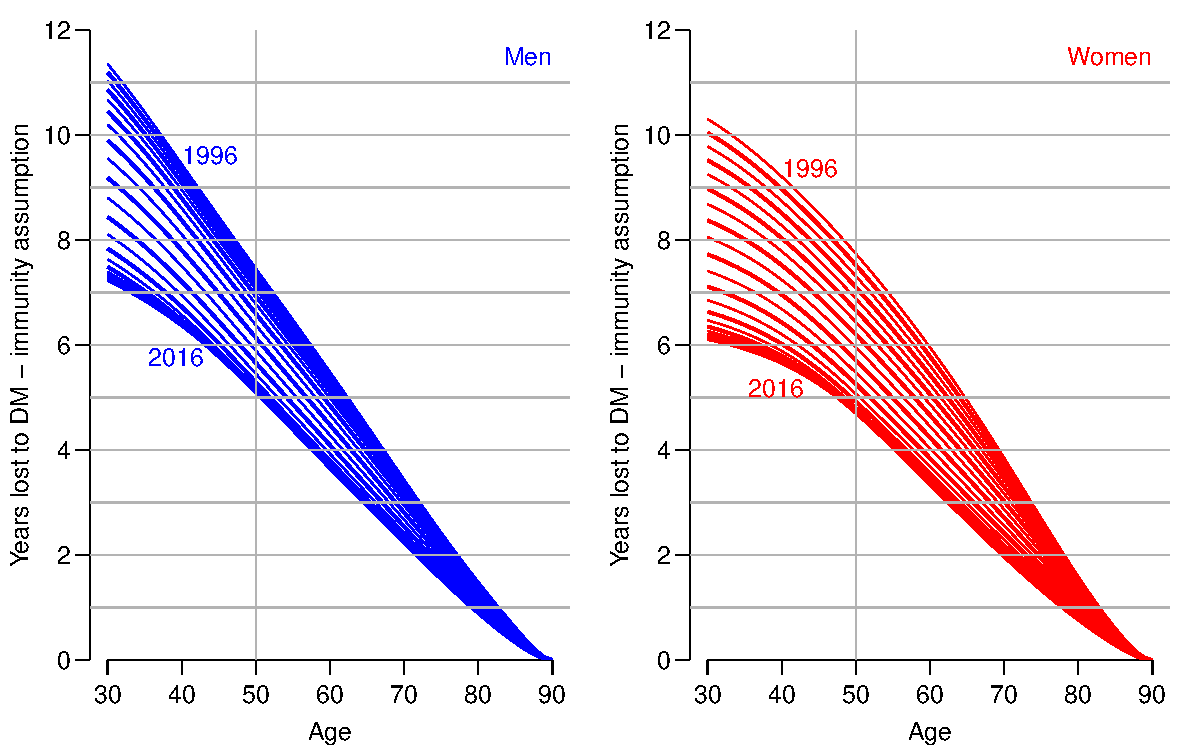
\includegraphics[width=\textwidth]{05yll-imm}
  \caption{Years of life lost to DM: the difference in expected
    residual life time at different ages between persons with and
    without diabetes, assuming the persons without diabetes at a given
    age remain free from diabetes (immunity assumption --- not
    reasonable). The lines refer to date of evaluation; the top lines
    refer to 1996-1-1 the bottom ones to 2016-1-1. Blue curves are
    men, red women.}
  \label{fig:imm}
\end{figure}

\begin{figure}[h]
  \centering
  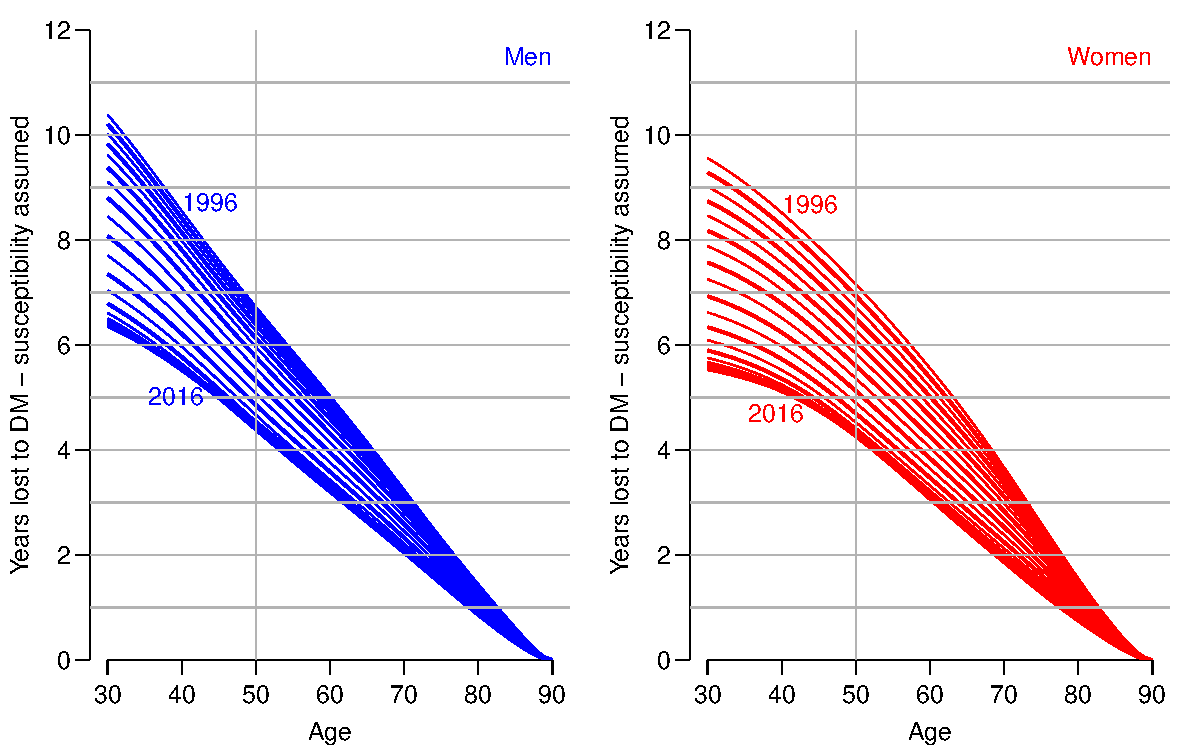
\includegraphics[width=\textwidth]{05yll-sus}
  \caption{Years of life lost to DM: the difference in expected
    residual life time at different ages between persons with and
    without diabetes, allowing the persons without diabetes at a given
    age to contract diabetes and thus be subject to higher
    mortality. The lines refer to date of evaluation; the top lines
    refer to 1996-1-1 the bottom ones to 2016-1-1. Blue curves are
    men, red women.}
  \label{fig:sus}
\end{figure}

\begin{figure}[h]
  \centering
  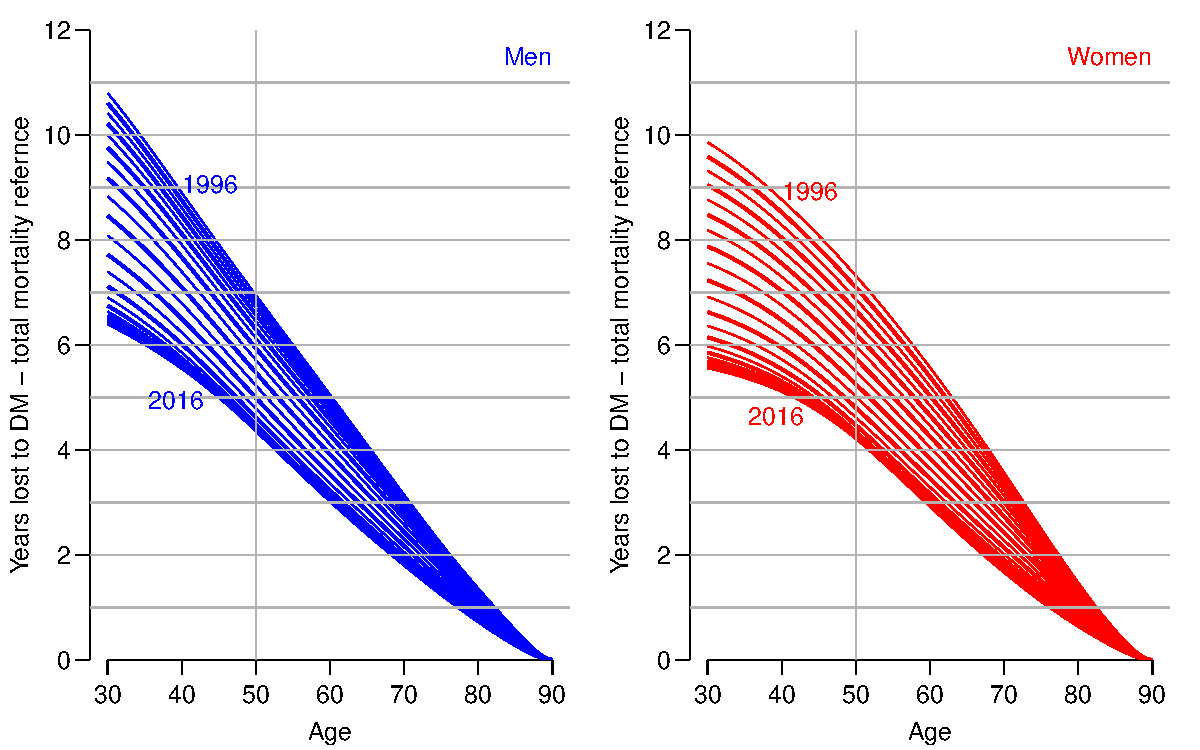
\includegraphics[width=\textwidth]{05yll-tot}
  \caption{Years of life lost to DM: the difference in expected
    residual life time at different ages between persons with and
    without diabetes. Allowance for susceptibility is approximated by
    using the total population mortality instead of non-DM
    mortality. The lines refer to date of evaluation; the top lines
    refer to 1996-1-1 the bottom ones to 2016-1-1. Blue curves are
    men, red women.}
  \label{fig:tot}
\end{figure}

From figure \ref{fig:sus} we see that for men aged 50 the years lost to
diabetes has decreased from 6.5 to 4.5 years
and for women from 4 to 4 years; so a greater improvement for women.

\begin{Schunk}
\begin{Soutput}
  Start time: 2025-10-06, 16:36:38 
    End time: 2025-10-06, 16:36:55 
Elapsed time: 0.29 minutes
\end{Soutput}
\end{Schunk}

\bibliographystyle{plain}

\begin{thebibliography}{1}

\bibitem{Carstensen.2007a}
B~Carstensen.
\newblock Age-{P}eriod-{C}ohort models for the {L}exis diagram.
\newblock {\em Statistics in Medicine}, 26(15):3018--3045, 2007.

\bibitem{Carstensen.2008c}
B~Carstensen, JK~Kristensen, P~Ottosen, and K~Borch-Johnsen.
\newblock The {D}anish {N}ational {D}iabetes {R}egister: {T}rends in incidence,
  prevalence and mortality.
\newblock {\em Diabetologia}, 51:2187--2196, 2008.

\end{thebibliography}

\addcontentsline{toc}{chapter}{References}

\end{document}
